\documentclass[varwidth=true, border=2pt]{standalone}

\usepackage{pgfplots}

\usepackage{amsmath}
\usepackage{tikz}
\renewcommand{\familydefault}{\sfdefault}


\def\y{-5}
\def\bb{4.2}
\def\m{.7}
\begin{document}
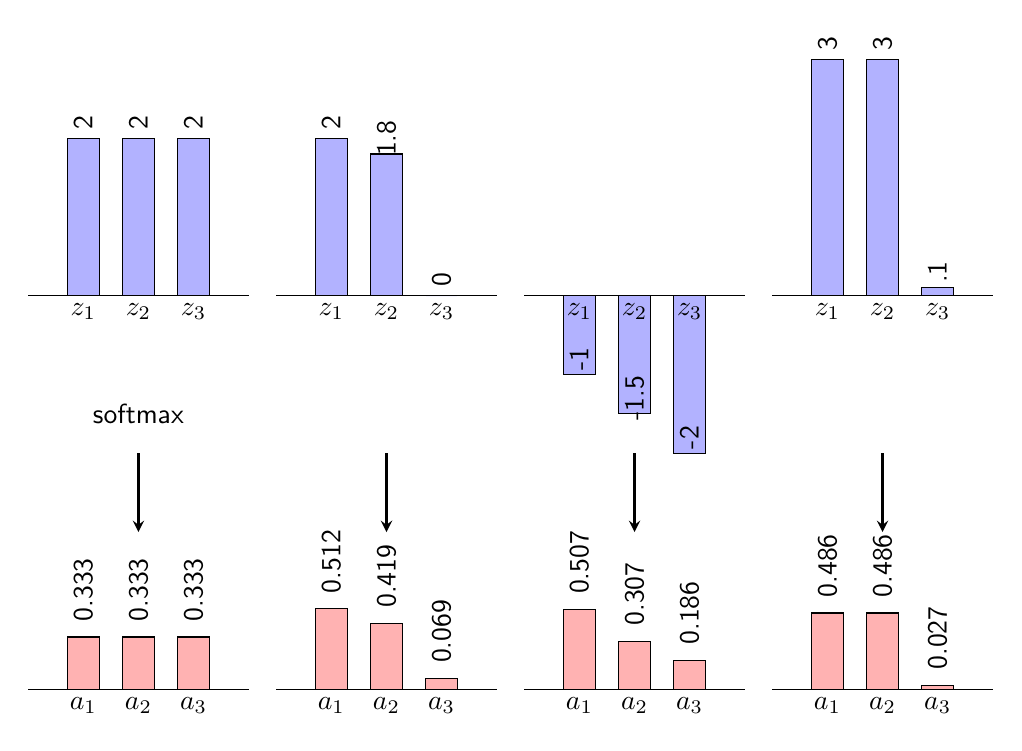
\begin{tikzpicture}[>= stealth]

\draw (0, 0) -- (4*\m, 0);
\draw (0, \y) -- (4*\m, \y);

\def\a{2}
\def\b{2}
\def\c{2}

\def\d{0.333}
\def\e{0.333}
\def\f{0.333}

\def\w{.2}
\def\t{.2}


\draw [fill = blue!30] (\m -\w, 0) rectangle (\m + \w, \a);
\draw [fill = blue!30] (2*\m -\w, 0) rectangle (2*\m + \w, \b);
\draw [fill = blue!30] (3*\m -\w, 0) rectangle (3*\m + \w, \c);

\node [rotate = 90] at (\m, \a+\t) {\a};
\node [rotate = 90] at (2*\m, \b+\t) {\b};
\node [rotate = 90] at (3*\m, \c+\t) {\c};
\node at (1*\m, -\t) {$z_1$};
\node at (2*\m, -\t) {$z_2$};
\node at (3*\m, -\t) {$z_3$};

\draw [fill = red!30] (1*\m -\w, \y) rectangle (1*\m + \w, \y + 2*\d);
\draw [fill = red!30] (2*\m -\w, \y) rectangle (2*\m + \w, \y + 2*\e);
\draw [fill = red!30] (3*\m -\w, \y) rectangle (3*\m + \w, \y + 2*\f);

\node [rotate = 90] at (1*\m, 2*\d+3*\t + \y) {\d};
\node [rotate = 90] at (2*\m, 2*\e+3*\t + \y) {\e};
\node [rotate = 90] at (3*\m, 2*\f+3*\t + \y) {\f};

\node at (1*\m, \y-\t) {$a_1$};
\node at (2*\m, \y-\t) {$a_2$};
\node at (3*\m, \y-\t) {$a_3$};

\node at (2*\m, -1.5) {softmax};
\draw [thick, ->] (2*\m, -2) -- (2*\m, -3);

\begin{scope}[xshift = 4.5*\m cm]
	\draw (0, 0) -- (4*\m, 0);
	\draw (0, \y) -- (4*\m, \y);

	\def\a{2}
	\def\b{1.8}
	\def\c{0}

	\def\d{0.512}
	\def\e{0.419}
	\def\f{0.069}

	\def\w{.2}
	\def\t{.2}


	\draw [fill = blue!30] (\m -\w, 0) rectangle (\m + \w, \a);
	\draw [fill = blue!30] (2*\m -\w, 0) rectangle (2*\m + \w, \b);
	\draw [fill = blue!30] (3*\m -\w, 0) rectangle (3*\m + \w, \c);

	\node [rotate = 90] at (\m, \a+\t) {\a};
	\node [rotate = 90] at (2*\m, \b+\t) {\b};
	\node [rotate = 90] at (3*\m, \c+\t) {\c};
	\node at (1*\m, -\t) {$z_1$};
	\node at (2*\m, -\t) {$z_2$};
	\node at (3*\m, -\t) {$z_3$};

	\draw [fill = red!30] (1*\m -\w, \y) rectangle (1*\m + \w, \y + 2*\d);
	\draw [fill = red!30] (2*\m -\w, \y) rectangle (2*\m + \w, \y + 2*\e);
	\draw [fill = red!30] (3*\m -\w, \y) rectangle (3*\m + \w, \y + 2*\f);

	\node [rotate = 90] at (1*\m, 2*\d+3*\t + \y) {\d};
	\node [rotate = 90] at (2*\m, 2*\e+3*\t + \y) {\e};
	\node [rotate = 90] at (3*\m, 2*\f+3*\t + \y) {\f};

	\node at (1*\m, \y-\t) {$a_1$};
	\node at (2*\m, \y-\t) {$a_2$};
	\node at (3*\m, \y-\t) {$a_3$};

	\draw [thick, ->] (2*\m, -2) -- (2*\m, -3);
\end{scope}

\begin{scope}[xshift = 9*\m cm]
	\draw (0, 0) -- (4*\m, 0);
	\draw (0, \y) -- (4*\m, \y);

	\def\a{-1}
	\def\b{-1.5}
	\def\c{-2}

	\def\d{0.507}
	\def\e{0.307}
	\def\f{0.186}

	\def\w{.2}
	\def\t{.2}


	\draw [fill = blue!30] (\m -\w, 0) rectangle (\m + \w, \a);
	\draw [fill = blue!30] (2*\m -\w, 0) rectangle (2*\m + \w, \b);
	\draw [fill = blue!30] (3*\m -\w, 0) rectangle (3*\m + \w, \c);

	\node [rotate = 90] at (\m, \a+\t) {\a};
	\node [rotate = 90] at (2*\m, \b+\t) {\b};
	\node [rotate = 90] at (3*\m, \c+\t) {\c};
	\node at (1*\m, -\t) {$z_1$};
	\node at (2*\m, -\t) {$z_2$};
	\node at (3*\m, -\t) {$z_3$};

	\draw [fill = red!30] (1*\m -\w, \y) rectangle (1*\m + \w, \y + 2*\d);
	\draw [fill = red!30] (2*\m -\w, \y) rectangle (2*\m + \w, \y + 2*\e);
	\draw [fill = red!30] (3*\m -\w, \y) rectangle (3*\m + \w, \y + 2*\f);

	\node [rotate = 90] at (1*\m, 2*\d+3*\t + \y) {\d};
	\node [rotate = 90] at (2*\m, 2*\e+3*\t + \y) {\e};
	\node [rotate = 90] at (3*\m, 2*\f+3*\t + \y) {\f};

	\node at (1*\m, \y-\t) {$a_1$};
	\node at (2*\m, \y-\t) {$a_2$};
	\node at (3*\m, \y-\t) {$a_3$};

	\draw [thick, ->] (2*\m, -2) -- (2*\m, -3);
\end{scope}


\begin{scope}[xshift = 13.5*\m cm]
	\draw (0, 0) -- (4*\m, 0);
	\draw (0, \y) -- (4*\m, \y);

	\def\a{3}
	\def\b{3}
	\def\c{.1}

	\def\d{0.486}
	\def\e{0.486}
	\def\f{0.027}

	\def\w{.2}
	\def\t{.2}


	\draw [fill = blue!30] (\m -\w, 0) rectangle (\m + \w, \a);
	\draw [fill = blue!30] (2*\m -\w, 0) rectangle (2*\m + \w, \b);
	\draw [fill = blue!30] (3*\m -\w, 0) rectangle (3*\m + \w, \c);

	\node [rotate = 90] at (\m, \a+\t) {\a};
	\node [rotate = 90] at (2*\m, \b+\t) {\b};
	\node [rotate = 90] at (3*\m, \c+\t) {\c};
	\node at (1*\m, -\t) {$z_1$};
	\node at (2*\m, -\t) {$z_2$};
	\node at (3*\m, -\t) {$z_3$};

	\draw [fill = red!30] (1*\m -\w, \y) rectangle (1*\m + \w, \y + 2*\d);
	\draw [fill = red!30] (2*\m -\w, \y) rectangle (2*\m + \w, \y + 2*\e);
	\draw [fill = red!30] (3*\m -\w, \y) rectangle (3*\m + \w, \y + 2*\f);

	\node [rotate = 90] at (1*\m, 2*\d+3*\t + \y) {\d};
	\node [rotate = 90] at (2*\m, 2*\e+3*\t + \y) {\e};
	\node [rotate = 90] at (3*\m, 2*\f+3*\t + \y) {\f};

	\node at (1*\m, \y-\t) {$a_1$};
	\node at (2*\m, \y-\t) {$a_2$};
	\node at (3*\m, \y-\t) {$a_3$};

	\draw [thick, ->] (2*\m, -2) -- (2*\m, -3);
\end{scope}
\end{tikzpicture}
\end{document}

% \documentclass[varwidth=true, border=2pt]{standalone}

% \usepackage{bchart}

% \begin{document}
%     \begin{bchart}[step=2, max = 2.5]
%         \bcbar{2}
%             \smallskip
%         \bcbar{0.1}
%             \smallskip
%             % \medskip
%         \bcbar{-1}
%     \end{bchart}
% \end{document}